\documentclass[11pt]{article}
\usepackage[margin=1in]{geometry}
\usepackage{amsmath}
\usepackage{booktabs}
\usepackage{graphicx}
\usepackage{circuitikz}
\definecolor{hl}{HTML}{EA580C}
\usepackage[hidelinks]{hyperref}
\usepackage{parskip}

\newcommand{\Vdet}{V_{\mathrm{det}}}
\newcommand{\Venv}{V_{\mathrm{env}}}
\newcommand{\Vbe}{V_{\mathrm{BE}}}
\newcommand{\Rtop}{R_{\mathrm{top}}}
\newcommand{\Rbot}{R_{\mathrm{bot}}}
\newcommand{\kO}{\,\mathrm{k\Omega}}

\title{Audio Visualizer: Calculation of the LED Loudness Ladder (STE)}
\author{Lucas Krippendorff}
\date{}

\begin{document}
\maketitle

\noindent
Each channel has ten LEDs. The LEDs come on in sequence when the sound
becomes louder. The circuit does not use a driver IC. It uses transistors,
resistors, and one half of an LM358 for each channel. This document gives
the calculation of the resistor values.

\begin{figure}[h]
\centering
\begin{circuitikz}[american, scale=0.82, transform shape]
  % envelope detector
  \draw (0,0) node[left]{audio in} to[C, l=$1\,\mu$F] (1.9,0) to[D, l=BAT85] (3.5,0);
  \draw (3.5,0) node[circ]{} node[above=4pt, xshift=8pt]{$\Vdet$};
  \draw (3.5,0) to[C, l_=$10\,\mu$F] (3.5,-2.2) node[ground]{};
  \draw (3.5,0) -- (5.1,0);
  \draw (5.1,0) node[circ]{} to[R, l_=22k] (5.1,-2.2) node[ground]{};
  % op amp, non-inverting x2.1 (flipped: + on top, feedback below)
  \node[op amp, noinv input up, anchor=+] (oa) at (8.1,0) {};
  \node[above=1pt] at (oa.north) {LM358};
  \draw (5.1,0) -- (oa.+);
  \draw (oa.-) -- ++(-0.4,0) coordinate(fb) -- ++(0,-0.9) coordinate(fb3) node[circ]{};
  \draw (fb3) to[R, l_=10k] ++(0,-1.6) node[ground]{};
  \draw (oa.out) -- ++(0.4,0) coordinate(o1) node[circ]{};
  \draw (fb3) to[R, l_=11k] (fb3 -| o1) -- (o1);
  \draw (o1) to[short, -*] ++(0.7,0) coordinate(bus) node[above=2pt]{$\Venv$};
  % divider + stage
  \draw (bus) to[R, l=$R_{\mathrm{top},k}$] ++(2.5,0) coordinate(b) node[circ]{};
  \node[above=4pt, xshift=6pt, color=hl] at (b) {$\Vbe$};
  \draw (b) to[R, l_=$R_k$] ++(0,-2.2) node[ground]{};
  \draw (b) -- ++(0.8,0) node[npn, anchor=B] (q) {};
  \node[right=6pt, yshift=-10pt] at (q.east) {MMBT3904};
  \draw (q.E) -- ++(0,-0.3) node[ground]{};
  \draw (q.C) ++(0,3.2) node[vcc]{+12\,V} to[R, l=3.3k] ++(0,-1.7) to[full led, l=LED] (q.C);
\end{circuitikz}
\caption{One channel: the front end and one of the ten ladder stages. The
divider pair $R_{\mathrm{top},k}$/$R_k$ is different for each stage. LED $k$
comes on when the base voltage is $\Vbe$. The threshold $V_k$ is not a node.
It is the $\Venv$ value that puts the base at $\Vbe$.}
\end{figure}

\section*{The loudness voltage}

The audio signal is AC. The ladder needs a DC voltage that follows the
volume. The $1\,\mu$F capacitor connects the signal to the detector. The
Schottky diode changes the signal to DC. The $10\,\mu$F capacitor holds the
peak voltage. The $22\kO$ resistor discharges the capacitor slowly
($\tau = 22\kO \times 10\,\mu\mathrm{F} \approx 0.22$\,s). This voltage is
$\Vdet$.

I set the clip level to $\Vdet = 5$\,V. This value is an estimate. The
speakers can supply a maximum of 6\,V. But the Schottky diode decreases the
voltage by approximately 0.3\,V. The other components in the signal path
also decrease the voltage. The display is only decorative. Thus a small
error in this value has no effect.

\section*{Logarithmic spacing}

Human hearing is logarithmic. Two loudness steps are equal when the two
voltage ratios are equal. Equal voltage steps do not give this result. Thus
the thresholds have equal spacing in dB. The LM3915 bar-driver IC uses the
same method. The range is 30\,dB. There are 13 steps of 2.5\,dB:
\begin{equation}
L_k = -30 + 2.5\,(k-1)\ \mathrm{dB}, \qquad
V_k = V_{\mathrm{fs}} \cdot 10^{L_k/20}.
\end{equation}

\section*{The gain stage}

The maximum detector voltage is 5\,V. The board operates from a 12\,V
supply. The maximum output of an LM358 on 12\,V is approximately 10.5\,V.
Thus I set the gain to $A = 10.5/5 = 2.1$. The resistors give this gain:
$A = 1 + 11\mathrm{k}/10\mathrm{k}$. Full scale and the clip level are the
same voltage. This was my intention. Thus the top LED shows clipping. The op
amp also isolates the detector. The ladder gets its current from the op amp,
not from the peak-hold capacitor.

\section*{One transistor and three resistors for each LED}

Each stage has an NPN transistor. The emitter connects to ground. The LED
and its $3.3\kO$ resistor connect to the collector. Two more resistors make
the base divider. The divider sets the voltage at which the stage comes on:
\begin{equation}
V_k = \Vbe\left(1 + \frac{\Rtop}{R_k}\right)
\quad\Longrightarrow\quad
\frac{\Rtop}{R_k} = \frac{V_k}{\Vbe} - 1.
\label{eq:rk}
\end{equation}
A divider can only decrease a voltage. Thus a threshold below
$\Vbe \approx 0.65$\,V is not possible. I found the number 13 by trial and
error. With 13 divisions, three thresholds (0.33, 0.44, 0.59\,V) are below
$\Vbe$. The ten LEDs that remain are the LEDs I wanted. The usable range is
$-22.5$\,dB to 0\,dB.

I adjust the top resistor and the bottom resistor for each stage. Two free
values give a smaller error. They also give more options from the JLCPCB
basic catalog. Each part that is not in the basic catalog adds a fee. The
error column shows the difference between the real threshold and the ideal
$V_k$. The maximum error is 1.4\%. Adjacent thresholds are 33\,\% apart.
Thus the LEDs always come on in the correct sequence:

\begin{center}
\begin{tabular}{c r r r r r r}
\toprule
LED & $L_k$ & ideal $V_k$ & $\Rtop$ & $R_k$ & threshold & error \\
\midrule
1  & $-22.5$\,dB & 0.787\,V  & $10\kO$  & $47\kO$  & 0.788\,V  & $+0.1\%$ \\
2  & $-20.0$\,dB & 1.050\,V  & $20\kO$  & $33\kO$  & 1.044\,V  & $-0.6\%$ \\
3  & $-17.5$\,dB & 1.400\,V  & $27\kO$  & $24\kO$  & 1.381\,V  & $-1.4\%$ \\
4  & $-15.0$\,dB & 1.867\,V  & $22\kO$  & $12\kO$  & 1.842\,V  & $-1.4\%$ \\
5  & $-12.5$\,dB & 2.490\,V  & $6.8\kO$ & $2.4\kO$ & 2.492\,V  & $+0.1\%$ \\
6  & $-10.0$\,dB & 3.320\,V  & $10\kO$  & $2.4\kO$ & 3.358\,V  & $+1.1\%$ \\
7  & $-7.5$\,dB  & 4.428\,V  & $27\kO$  & $4.7\kO$ & 4.384\,V  & $-1.0\%$ \\
8  & $-5.0$\,dB  & 5.905\,V  & $22\kO$  & $2.7\kO$ & 5.946\,V  & $+0.7\%$ \\
9  & $-2.5$\,dB  & 7.874\,V  & $30\kO$  & $2.7\kO$ & 7.872\,V  & $-0.0\%$ \\
10 & $0.0$\,dB   & 10.500\,V & $15\kO$  & $1\kO$   & 10.400\,V & $-1.0\%$ \\
\bottomrule
\end{tabular}
\end{center}

Each collector resistor is
$R_C = (12 - 2.0 - 0.2)\,\mathrm{V} / 3\,\mathrm{mA} \approx 3.3\kO$. This
sets the LED current to approximately 3\,mA. The board has two equal
channels, one left and one right.

\begin{figure}[h]
\centering
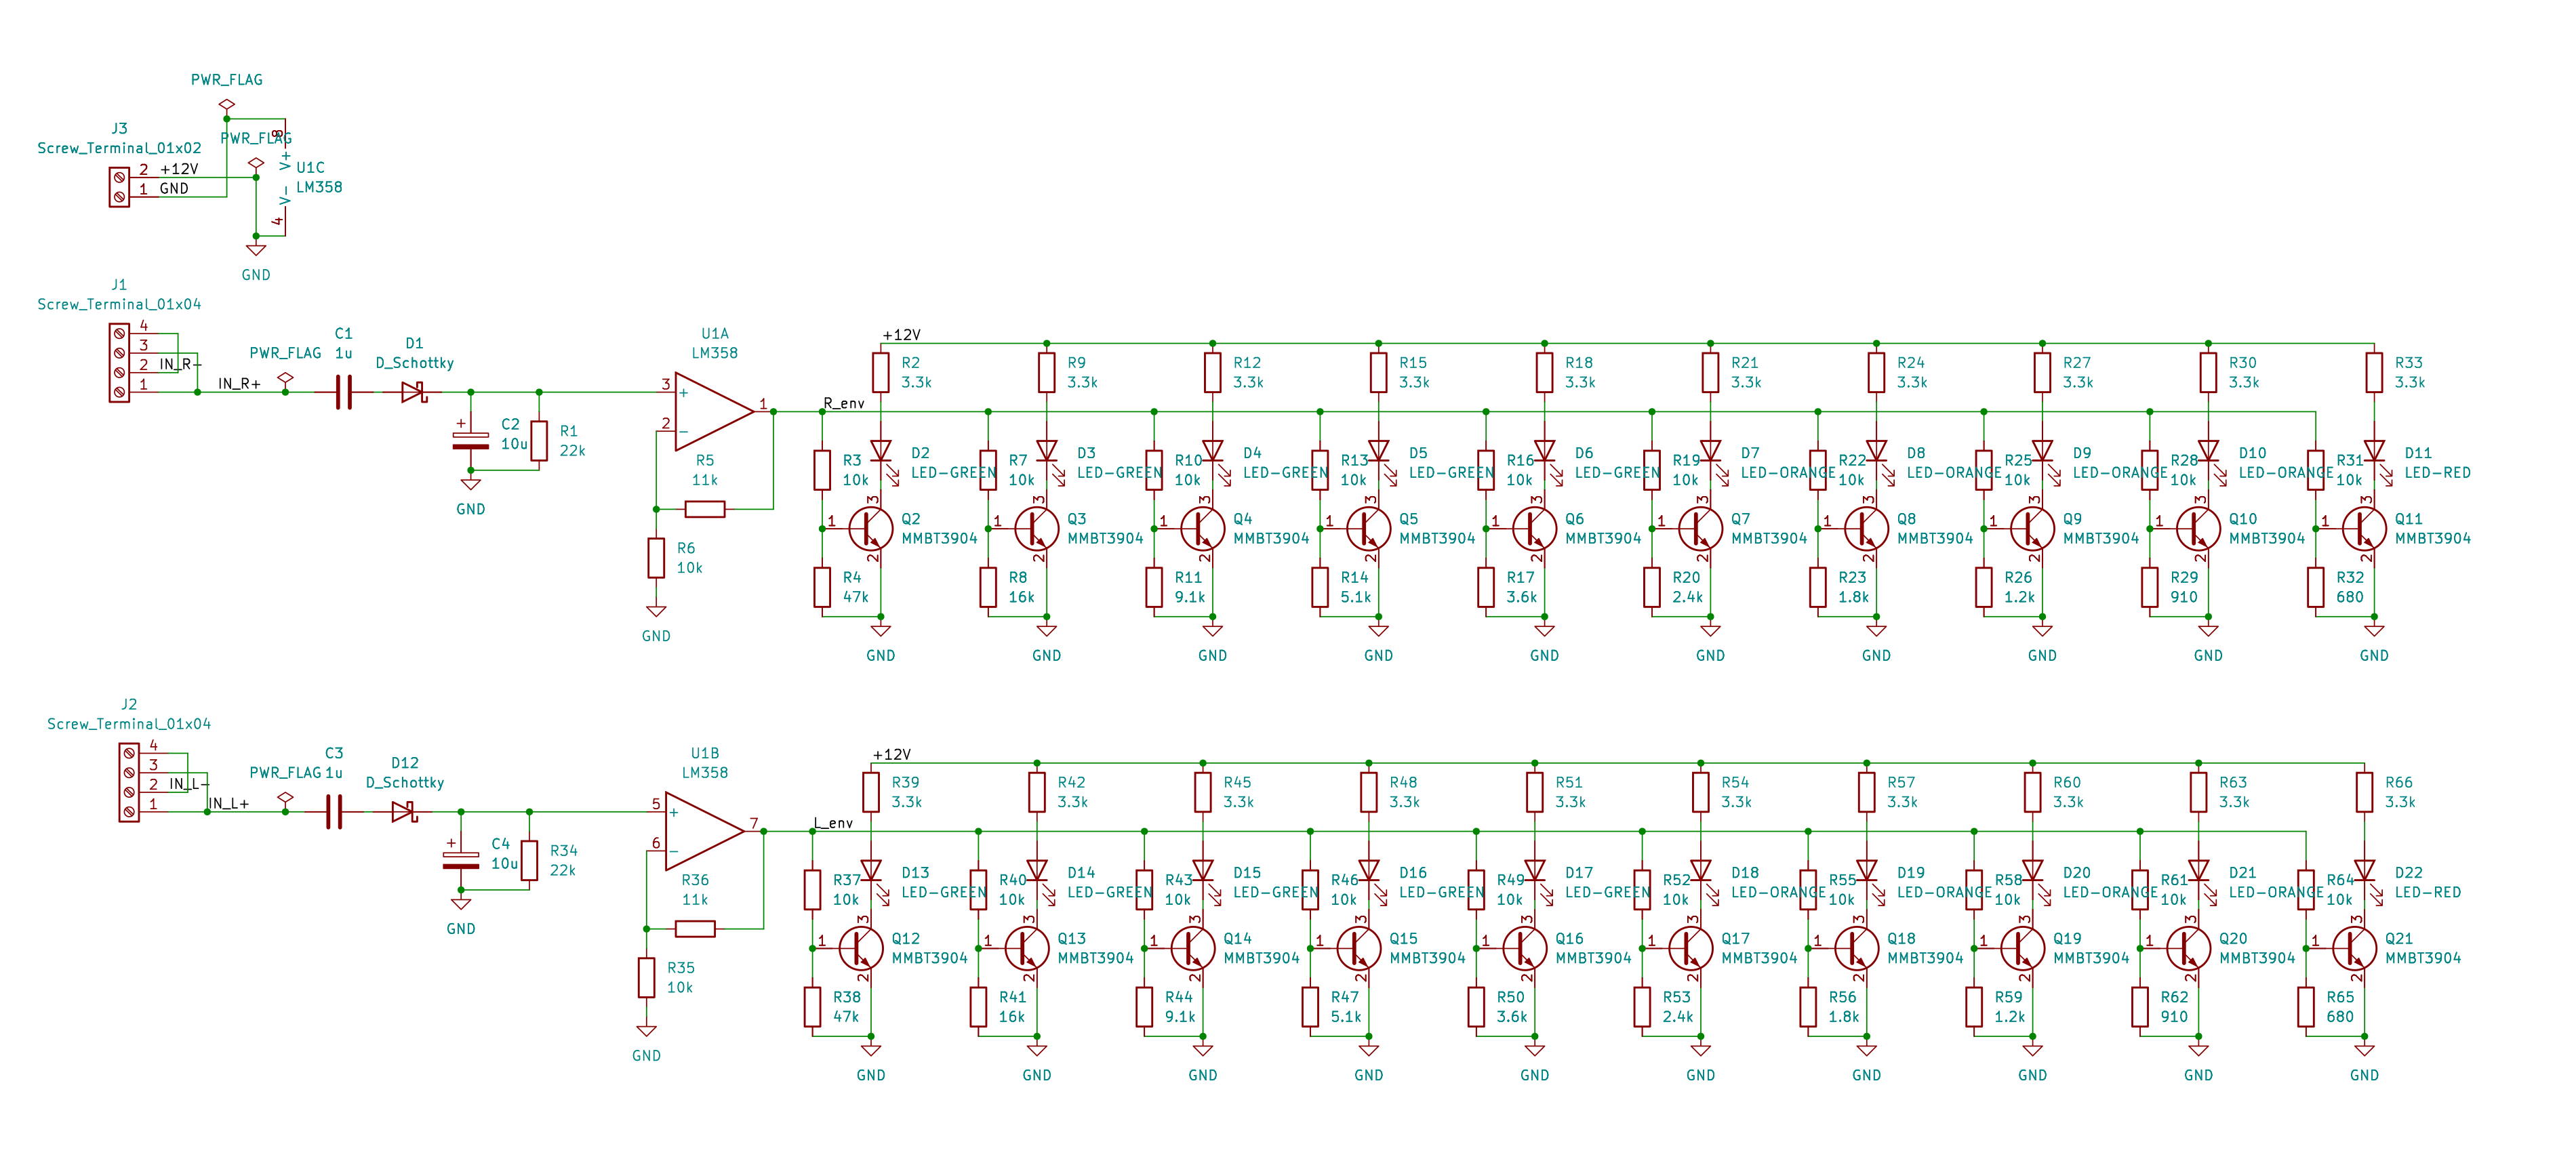
\includegraphics[width=\textwidth]{schematic_kicad.png}
\caption{The full schematic. Each half of the LM358 operates one ten-stage
ladder.}
\end{figure}

\begin{figure}[h]
\centering
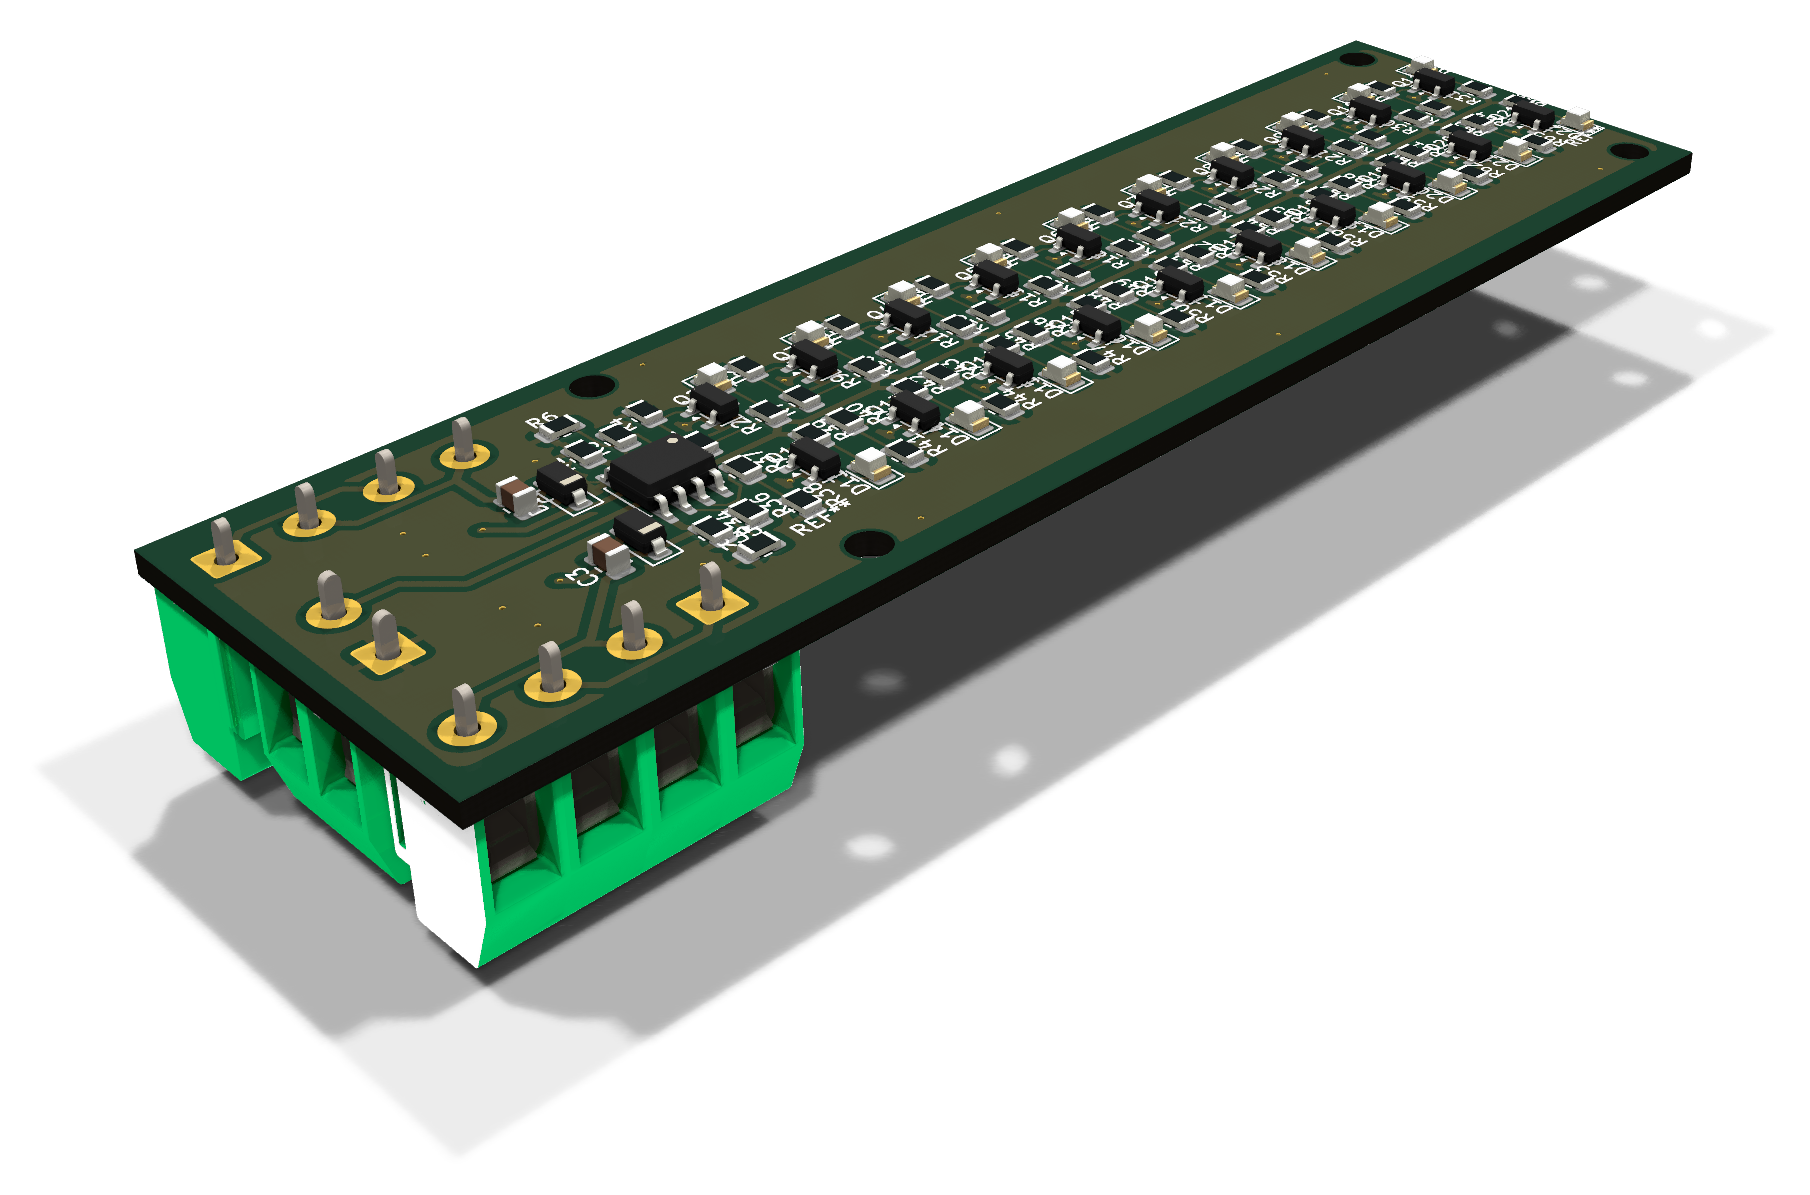
\includegraphics[width=0.62\textwidth]{render_corner.png}\\[6pt]
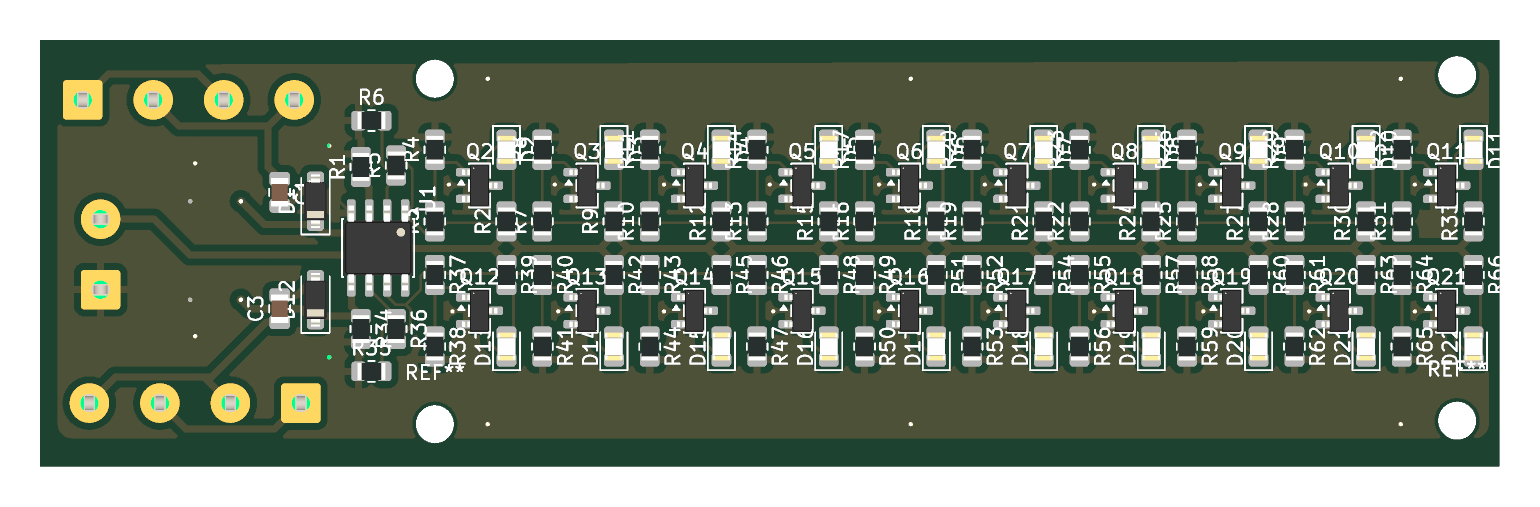
\includegraphics[width=0.85\textwidth]{render_top.png}
\caption{The V1 board. It has two channels of ten LEDs each.}
\end{figure}

\end{document}
